%%
%  ******************************************************************************
%  * #file    Szablon_raportu_EN_Latex.tex
%  * #author  Adrian Wójcik   adrian.wojcik(at)put.poznan.pl
%  *          
%  * #commit  Patryk Kościk   koscikpatryk(at)gmail.com
%  *          Modified the template for Projekt przejsciowy purposes          
%  *          
%  *
%  * #commit  Patryk Kościk   koscikpatryk(at)gmail.com
%  *          Zupełnie przewrócono na łeb formatke po taktycznym wyjasnieniu          
%  *          
%  * #version 1.1
%  * #date    09-Mar-2022
%  * #brief   PROJPRZEJ
%  *
%  ******************************************************************************
%%  
\documentclass[11pt, a4paper]{article}

\usepackage{SM_template}

% Wypełnijcie te dyrektywy zgodnie z waszym tematem
%
% \lab      -> NAZWA CZUJNIKA,          np.: 'DHT22'
% \comment  -> Króciutki opis co to,    np.: 'Cyfrowy czujnik temperatury'
% \author   -> Autor dokumentu          np.: Patryk Kościk
%
% Pamiętajcie o zmianie ścieżki w \addbibresourcue (!)

\lab{Moduł HW-596 (BMP180)}
\comment{Cyfrowy czujnik ciśnienia i temperatury}
\author{Jakub Grzesiak}
\addbibresource{bib/BMP180.bib}

%
% Początek dokumentu
%
\begin{document}

%
% Strona tytułowa
%
\mainpage{BMP180/zdj_modułu/BMP180.jpg}
\newpage

\section*{Opis elementu}
HW-596 to moduł którego głównym elementem jest cyfrowy czujnik ciśnienia i temperatury BMP180 firmy Bosch. Dzięki pomiarowi ciśnienia można pośrednio obliczyć także wysokość, na jakiej znajduje się czujnik. Dodatkowo, w module zamontowano stabilizator napięcia 662K, który obniża napięcie zasilające bezpośrednio czujnik BMP180. Działanie czujnika opiera się na efekcie piezorezystywnym. Polega ono na zmianie rezystancji elektrycznej elementu pod wpływem działającej siły. Komunikacja z zewnętrznymi układami odbywa się przy pomocy szeregowego, dwukierunkowego protokołu I$^2$C.
Moduł HW-596 może znaleźć zastosowanie w takich urządzeniach jak: telefony komórkowe, nawigacje GPS czy stacje pogodowe.
Na rysunku (\ref{fig:_bmp180_pinout}) przedstawiono moduł wraz z pinoutem.

%%%%%%%%%%%%%%%%%%%%%%%%%  TWO IMAGES SIDE BY SIDE  %%%%%%%%%%%%%%%%%%%%%%%%%%%%%
\vspace{0.25cm}
\begin{figure}[h]
\centering
%%%%%%%%%%%%%%%%%%%%%%%%%%%%%%%%%%%%%%%%%%%%%%%%%%%%%%%%%%%%%%%%%%%%%%%%%%%%%%%%%
\begin{subfigure}{.5\textwidth}
\centering
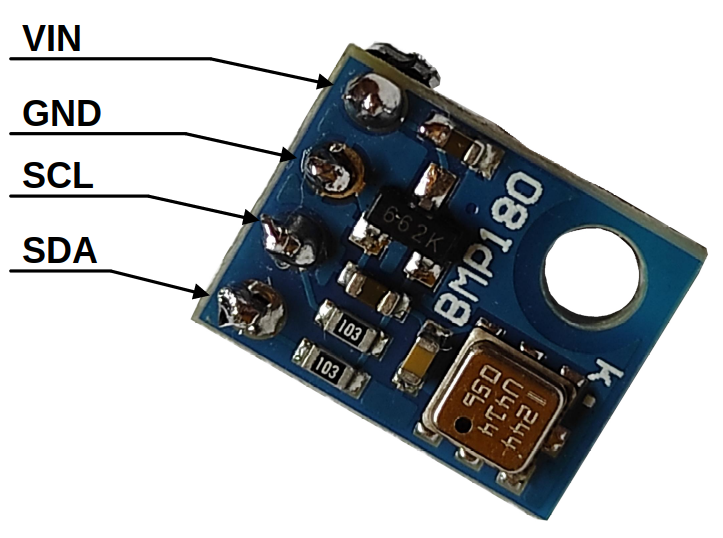
\includegraphics[width=0.7\linewidth]{fig/BMP180/zdj_modułu/bmp180_pinout.png}
\caption{Fizyczna budowa nadajnika wraz z pinoutem}
\label{fig:_bmp180_pinout}
\end{subfigure}%
%%%%%%%%%%%%%%%%%%%%%%%%%%%%%%%%%%%%%%%%%%%%%%%%%%%%%%%%%%%%%%%%%%%%%%%%%%%%%%%%%
\begin{subfigure}{.5\textwidth}
\centering
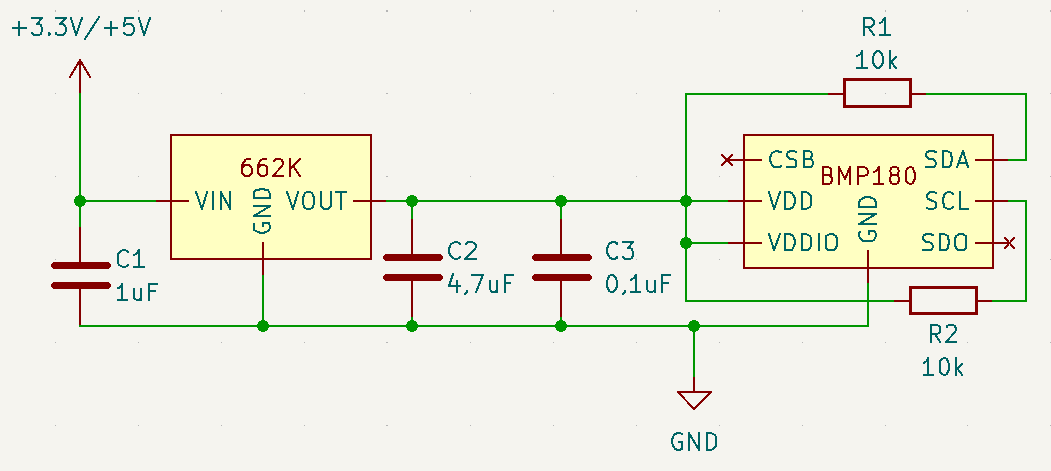
\includegraphics[width=1\linewidth]{fig/BMP180/polaczenie_modulu/schematic.png}
\caption{Schemat elektryczny modułu}
\label{fig:_schematic}
\end{subfigure}
%%%%%%%%%%%%%%%%%%%%%%%%%%%%%%%%%%%%%%%%%%%%%%%%%%%%%%%%%%%%%%%%%%%%%%%%%%%%%%%%%
% \caption{PODPIS}
\label{fig:element}
\end{figure}
\vspace{0.25cm}
%%%%%%%%%%%%%%%%%%%%%%%%%  TWO IMAGES SIDE BY SIDE  %%%%%%%%%%%%%%%%%%%%%%%%%%%%%

% \subsection{Opis modułu} REPLACE SUBSECTION WITH 1CM VSPACE
Moduł może być zasilanyn napięciami z zakresu $1,8V DC - 5V DC$. Zakres ciśnienia, jakie może zmierzyć czujnik to $300hPa - 1100hPa$ przy rozdzielczości $0,01hPa$, a zakres pośrednio liczonej wysokości nad poziomem morza wynosi od $-500m$ do $9000m$. Zakres temperatur od $-40^\circ C $ do $+85^\circ C $ przy rozdzielczości $0,1^\circ C $.
\\  \\
Schematy budowy wewnętrznej modułu przedstawiono na schemacie (\ref{fig:_schematic}). Rezystory R1 i R2 są rezystorami podciągającymi linie SDA i SCL do zasilania (ang pull-up resistors). Kondensator C1 pełni rolę filtru zewnętrznego napięcia zasilającego, a kondensator C2 i C3 filtrują napięcie wyjściowe ze stabilizatora napięcia 662K.

\vspace{0.25cm}
\begin{figure}[h]
    \centering
    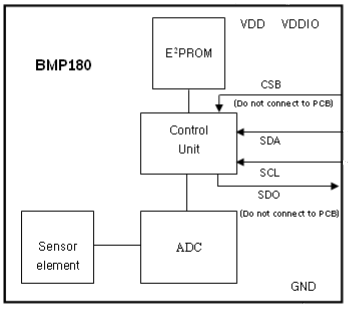
\includegraphics[width=.45\linewidth]{fig/BMP180/działanie_ukladu/bmp_block.png}
    \caption{Diagram blokowy budowy czujnika \cite{Bosch:BMP180}}
    \label{fig:_schemat_blok}
\end{figure}
\vspace{0.25cm}

Budowa wewnętrzna czujnika BMP180 została przedstawiona na diagramie blokowym (\ref{fig:_schemat_blok}). Napięcie mierzone na elementach o rezystancji zmiennej pod wpływem ciśnienia i pod wpływem temperatury konwertowane jestpoprzez przetwornik analogowo-cyfrowy (ADC). Pamięć E$^2$PROM przechowuje 176 bitów wykorzystywanych w kalibracji czujnika i kompensacji offsetów. Jednostka kontrolna steruje wymianą danych przy użyciu protokołu I$^2$C.
\\ 
Do konwersji ciśnienia na wysokość należy użyć wzoru (\ref{fig:_bmp180_formula}), w którym $p_0$ to ciśnienie atmosferyczne na poziomie morza równe $1013,25hPa$, a $p$ to aktualna wartość ciśnienia odczytana przez czujnik w $Pa$. Wykres (\ref{fig:_altitude}) przedstawia zależność wysokiści od ciśnienia atmosferycznego.

%%%%%%%%%%%%%%%%%%%%%%%%%  TWO IMAGES SIDE BY SIDE  %%%%%%%%%%%%%%%%%%%%%%%%%%%%%
\vspace{0.25cm}
\begin{figure}[h]
\centering
%%%%%%%%%%%%%%%%%%%%%%%%%%%%%%%%%%%%%%%%%%%%%%%%%%%%%%%%%%%%%%%%%%%%%%%%%%%%%%%%%
\begin{subfigure}{.5\textwidth}
\centering
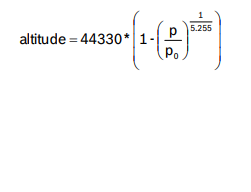
\includegraphics[width=0.6\linewidth]{fig/BMP180/działanie_ukladu/formula.png}
\caption{Wzór do obliczenia wysokości \cite{Bosch:BMP180}}
\label{fig:_bmp180_formula}
\end{subfigure}%
%%%%%%%%%%%%%%%%%%%%%%%%%%%%%%%%%%%%%%%%%%%%%%%%%%%%%%%%%%%%%%%%%%%%%%%%%%%%%%%%%
\begin{subfigure}{.5\textwidth}
\centering
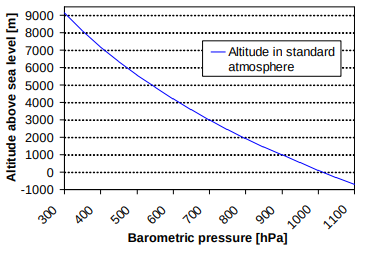
\includegraphics[width=0.84\linewidth]{fig/BMP180/działanie_ukladu/altitude.png}
\caption{Zależność wysokości od ciśnienia atmosferycznego \cite{Bosch:BMP180}}
\label{fig:_altitude}
\end{subfigure}
%%%%%%%%%%%%%%%%%%%%%%%%%%%%%%%%%%%%%%%%%%%%%%%%%%%%%%%%%%%%%%%%%%%%%%%%%%%%%%%%%
% \caption{PODPIS}
\label{fig:element}
\end{figure}
\vspace{0.25cm}
%%%%%%%%%%%%%%%%%%%%%%%%%  TWO IMAGES SIDE BY SIDE  %%%%%%%%%%%%%%%%%%%%%%%%%%%%%


\\ \\
Protokół komunikacyjny I$^2$C (ang. Inter-Integrated Circuit) jest protokołem synchronicznym, dwukierunkowym typu master-slave. Korzysta on z dwóch dwukierunkowych linii:
\begin{itemize}
  \item $SCL$ - Serial Clock Line - linia przesyłu danych
  \item $SDA$ - Serial Data Line - taktująca linia zegarowa
\end{itemize}
Ramkę protokołu I$^2$C przedstawiono na rysunku (\ref{fig:_i2c_frame}):

\vspace{0.25cm}
\begin{figure}[h]
    \centering
    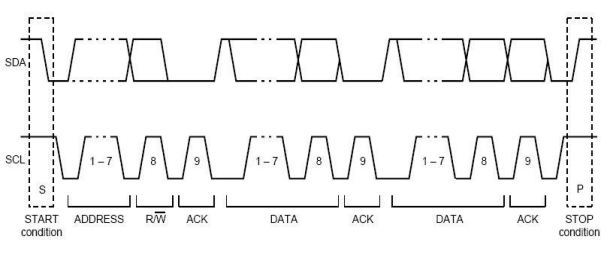
\includegraphics[width=.7\linewidth]{fig/BMP180/działanie_ukladu/i2c_frame.png}
    \caption{Schemat budowy ramki protokołu I$^2$C \cite{Bosch:BMP180}}
    \label{fig:_i2c_frame}
\end{figure}
\vspace{0.25cm}
Aby transmisja wystartowała, linia $SCL$ musi być w stanie wysokim, a na linii $SDA$ musi wystąpić zbocze opadające. Następnie wysyłane jest 7 bitów określających adres urządzenia, bit R/W ('0', gdy master wysyła dane do slave'a - Write lub '1' gdy master chce odczytać dane od slave'a - Read). Gdy slave rozpozna, że jest adresowany, w dziewiątym cyklu zegara wysyła sygnał $ACK$ jako niski stan logiczny na linii $SDA$. Następnie przesyłany jest bajt danych, po którym ponownie następuje potwierdzenie transmisji $ACK$. Aby zakończyć transmisję, linia $SCL$ musi być w stanie wysokim, a na linii $SDA$ musi wystąpić zbocze narastające.
\\
Dane o temperaturze z czujnika BMP180 zajmują w ramce protokołu I$^2$C jedno słowo, czyli 16 bitów (inaczej 2 bajty), a dane o ciśnieniu zajmują od 16 do 19 bitów. Należy pamiętać także o maksymalnej częstotliwości taktującego sygnału zegarowego, która w przypadku czujnika BMP180 wynosi $3,4MHz$.



\section{Użycie czujnika}
Moduł posiada 4 wyprowadzenia - 2 zasilające i 2 sygnałowe interfejsu komunikacyjnego I$^2$C. Na rys. (\ref{fig:_bmp180_pinout}) przedstawiono oznaczenia wyprowadzeń rzeczywistego czujnika. Działanie czujnika można zweryfikować z użyciem mikrokontrolera. W poniższym przykładzie użyto płytki rozwojowej STM32 NUCLEO-F767ZI. Układ połączeń przedstawiony na rysunku (\ref{fig:_polaczenie_ukladu}) oraz program dla płytki NUCLEO-F746ZG będzie identyczny. Kod skonfigurowano tak, aby przez komunikację szeregową UART wysyłana była co $0,5s$ aktualna wartość ciśnienia i temperatury odczytana z czujnika. Dodatkowo, działanie programu fizycznie sygnalizuje miganie niebieskiej, wbudowanej w płytkę diody LD2.

\vspace{0.25cm}
\begin{figure}[h]
    \centering
    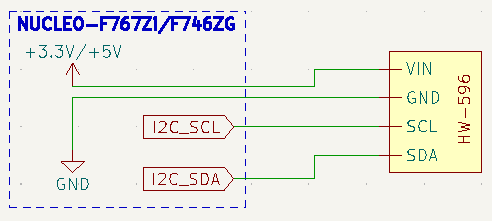
\includegraphics[width=0.7\textwidth]{fig/BMP180/polaczenie_modulu/nucleo_con.png}
    \caption{Połączenie układu z mikroprocesorem}
    \label{fig:_polaczenie_ukladu}
\end{figure}
\vspace{0.25cm}

Poniżej zaprezentowano zdjęcie rzeczywistego układu oraz jego przykładowe odpowiedzi z ciśnieniem, temperaturą i wysokością wysyłane poprzez UART. Kod zaimplementowany na mikroprocesorze zawarty jest w \texttt{Suplement \#1}.

% TUTAJ FOTY ODNOSNIE TEGO
%%%%%%%%%%%%%%%%%%%%%%%%%  TWO IMAGES SIDE BY SIDE  %%%%%%%%%%%%%%%%%%%%%%%%%%%%%
\vspace{0.25cm}
\begin{figure}[h]
\centering
%%%%%%%%%%%%%%%%%%%%%%%%%%%%%%%%%%%%%%%%%%%%%%%%%%%%%%%%%%%%%%%%%%%%%%%%%%%%%%%%%
\begin{subfigure}{.5\textwidth}
\centering
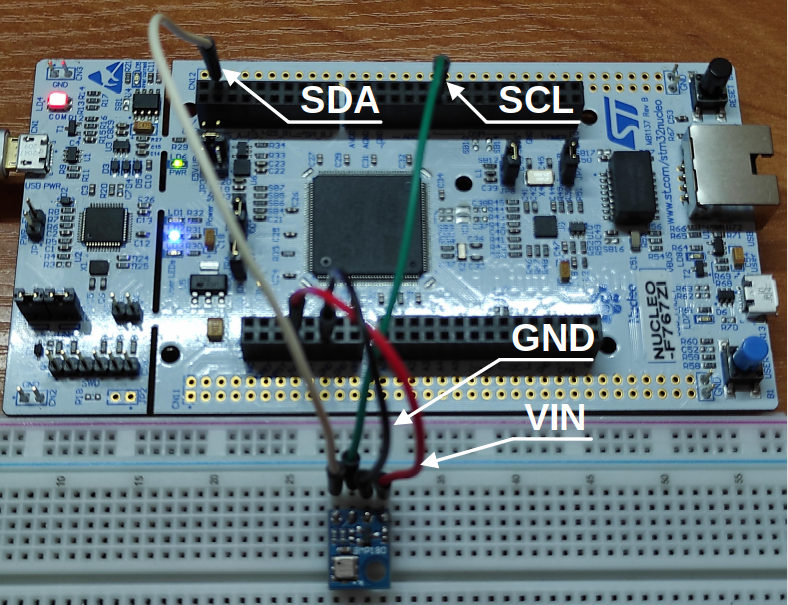
\includegraphics[width=0.8\linewidth]{fig/BMP180/zdj_modułu/nucleo_con.png}
\caption{Fizyczne połączenie układu z mikroprocesorem}
\label{fig:_nucleo_con}
\end{subfigure}%
%%%%%%%%%%%%%%%%%%%%%%%%%%%%%%%%%%%%%%%%%%%%%%%%%%%%%%%%%%%%%%%%%%%%%%%%%%%%%%%%%
\begin{subfigure}{.5\textwidth}
\centering
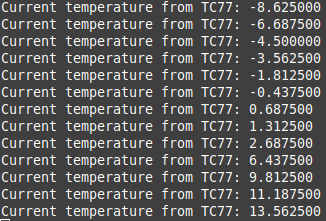
\includegraphics[width=1\linewidth]{fig/BMP180/działanie_ukladu/uart.png}
\caption{Przykładowe odczyty temperatury, ciśnienia i wysokości}
\label{fig:_altitude}
\end{subfigure}
%%%%%%%%%%%%%%%%%%%%%%%%%%%%%%%%%%%%%%%%%%%%%%%%%%%%%%%%%%%%%%%%%%%%%%%%%%%%%%%%%
% \caption{PODPIS}
\label{fig:element}
\end{figure}
\vspace{0.25cm}
%%%%%%%%%%%%%%%%%%%%%%%%%  TWO IMAGES SIDE BY SIDE  %%%%%%%%%%%%%%%%%%%%%%%%%%%%%
Dodatkowo działanie układu przedstawiono na załączonym w \texttt{Suplement Wideo} materiale 
wideo.

\newpage
\printbibliography[heading=bibintoc]

\end{document}